%
% main.tex -- Paper zum Thema Polynome
%
% (c) 2019 Hochschule Rapperswil
%
\chapter{Wavelets und polynomiale Signale\label{chapter:thema}}
\lhead{Wavelets und polynomiale Signale}
\begin{refsection}
\chapterauthor{Raphael Nestler}

In der Literatur zu Wavelets findet man die folgende Aussage zu Daubechies
Wavelets:
\begin{displayquote}[\cite{wikipedia:daubechies}]
For example, $D2$, with one vanishing moment, easily encodes polynomials of one
coefficient, or constant signal components. $D4$ encodes polynomials with two
coefficients, i.e.\ constant and linear signal components; and $D6$ encodes
3-polynomials, i.e.\ constant, linear and quadratic signal components.
\end{displayquote}
Ein Daubechies Wavelet mit $A$ verschwindenden Momenten und Filterlänge $N=2A$
soll also ein Polynom der Ordnung $A-1$ einfach darstellen können. Wir wollen
erörtern, was das nun in der Praxis genau bedeutet und welche Anwendungen es
ermöglicht.

\begin{figure}
    \centering
    % Filter mit 2 Ebenen

\usetikzlibrary{shapes,arrows}

\tikzset{%
  block/.style    = {draw, thick, rectangle, minimum height = 3em,
    minimum width = 3em},
  input/.style    = {coordinate}, % Input
  output/.style   = {coordinate} % Output
}
% Defining string as labels of certain blocks.
\newcommand{\suma}{\Large$+$}
\newcommand{\inte}{$\displaystyle \int$}
\newcommand{\derv}{\huge$\frac{d}{dt}$}

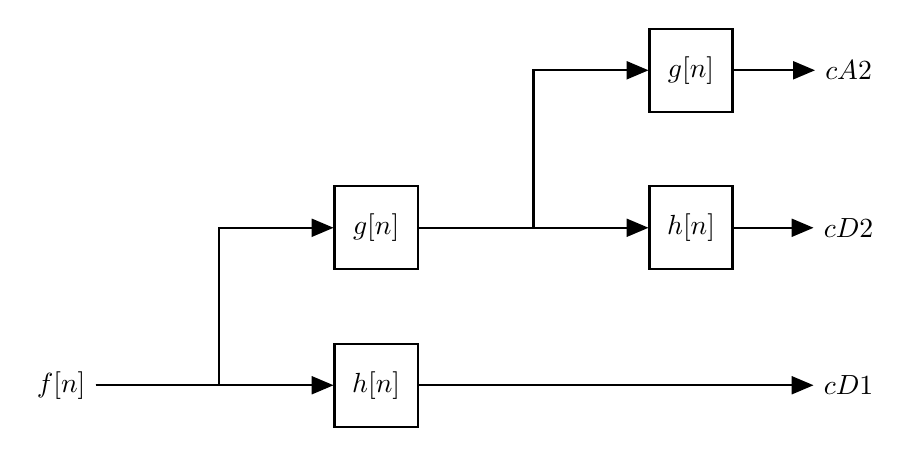
\begin{tikzpicture}[auto, thick, node distance=2cm, >=triangle 45]
\draw
	% Ebene 1
	node at (0,0)[name=in]{$f[n]$}
    node [input, right of=in](input1){}
	node [block, right of=input1] (h1) {$h[n]$}
	node [block, above of=h1] (g1) {$g[n]$}

	% Ebene 2
    node [input, right of=g1](input2){}
	node [block, right of=input2] (h2) {$h[n]$}
	node [block, above of=h2] (g2) {$g[n]$}

	% Ausgänge
    node [right of=g2](outg) {$cA2$}
    node [below of=outg](out2) {$cD2$}
    node [below of=out2](out1) {$cD1$}
;

    % Ebene 1
	\draw[->](in) -- node {}(h1);
	\draw[->](in) -- (input1) |- node {}(g1);
	\draw[->](h1) -- node {}(out1);

    % Ebene 2
	\draw[->](g1) -- node {}(h2);
	\draw[->](g1) -- (input2) |- node {}(g2);
	\draw[->](h2) -- node {}(out2);

	\draw[->](g2) -- node {}(outg);


\end{tikzpicture}
    \caption{Wavelet-Transformation als Filter\label{polynomials:filter}}
\end{figure}

Wir werden im folgenden Daubechies Wavelets mit $A$ verschwindenden Momenten
mit db$A$ bezeichnen. Auch werden wir die Wavelet-Transformation als Filter
betrachten wie in \autoref{haar:approximation:filter} beschrieben. Dabei werden
wir die Notation von Detail- und Approximationskoeffizienten verwenden. Die
Detailkoeffizienten auf Ebene $j$ ($cDj$) sind dabei der Ausgang des Hochpasses
$h$ und die Approximationskoeffizienten auf Ebene $j$ ($cAj$) der Ausgang des
Tiefpasses $g$.

Die Detailkoeffizienten auf Ebene $j$ entsprechen der Analyse mit einem $2^j$
skaliertem Mutterwavelet $\psi$ und die Approximationskoeffizienten der
entsprechenden Analyse mit einem Vaterwavelet $\varphi$.

Die Analysen und Simulationen wurden jeweils mittels Python~\cite{python} und im
speziellem dem PyWavelets~\cite{gregory_r_lee_2019_2634243} Paket durchgeführt.
Der dazu verwendete Code wurde in einem GitHub-Repository%
\footnote{\url{https://github.com/rnestler/mathsem-FS2019/tree/paper}}%
~\cite{polynomials:repo}
abgelegt. Zusätzlich sind auch interaktive Jupyter Notebooks abgelegt um den
Einfluss von verschiedenen Parametern auszuprobieren. Mittels
Binder%
\footnote{\url{https://mybinder.org/v2/gh/rnestler/mathsem-FS2019/paper}}%
~\cite{project_jupyter-proc-scipy-2018}
kann eine Online-Umgebung gestartet werden um diese Beispiele auszuführen.

\section{Analyse von polynomialen Signalen}
\rhead{Polynomiale Signale}

Wir werden als erstes die Signale in \autoref{polynomials:signals} mittels des db1
(Haar) Wavelets analysieren.

\begin{figure}
    \centering
    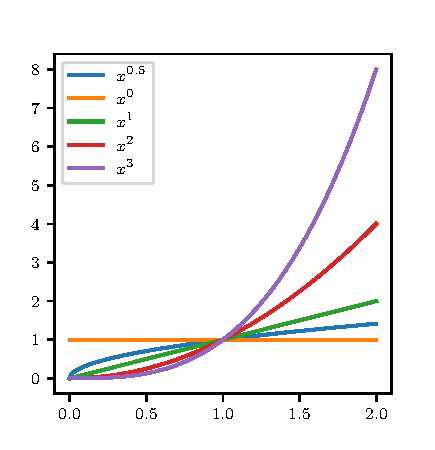
\includegraphics{papers/polynomials/images/polynomials_signals.pdf}
    \caption{Die verschiedenen zu analysierenden polynomialen Signale\label{polynomials:signals}}
\end{figure}

In~\autoref{polynomials:haar} sind die Approximations- und die Detailkoeffizienten
der Transformation zu sehen. Wir sehen, dass die Approximationskoeffizienten
uns das grobe Signal und im Fall von $x^0 = 1$ sogar das exakte Signal liefern. Die
Detailkoeffizienten scheinen uns etwas zu liefern was proportional zur ersten
Ableitung des Signals ist.

\begin{figure}
    \centering
    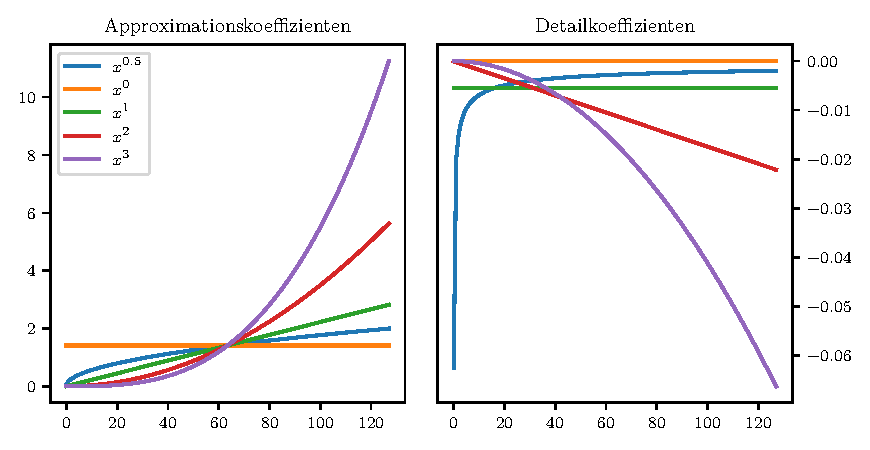
\includegraphics{papers/polynomials/images/polynomials_signals_db1.pdf}
    \caption{Analyse mit db1 (Haar) Wavelet\label{polynomials:haar}}
\end{figure}

In \autoref{polynomials:diff} sind zum Vergleich die Ableitungen der
verschiedenen Signale geben.

\begin{figure}
    \centering
    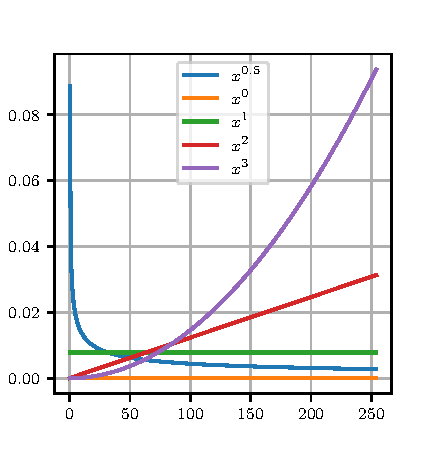
\includegraphics{papers/polynomials/images/polynomials_signals_diff.pdf}
    \caption{Ableitungen der Polynome\label{polynomials:diff}}
\end{figure}

Dieses Verhalten ist zu erwarten wenn man bedenkt, dass das Haar Wavelet
jeweils die Summe und die Differenz zweier benachbarter Samples analysiert.
Siehe dazu auch \autoref{haar:allwavelets:image} im Kapitel zum Haar Wavelet.

Nun stellt sich die Frage was passiert wenn wir Daubechies Wavelets mit mehr
verschwindenden Momenten zur Analyse einsetzen. In \autoref{polynomials:db2_3}
sind jeweils die Detailkoeffizienten der Analyse mit db1 und db2 Wavelet zu
sehen.

\begin{figure}
    \centering
    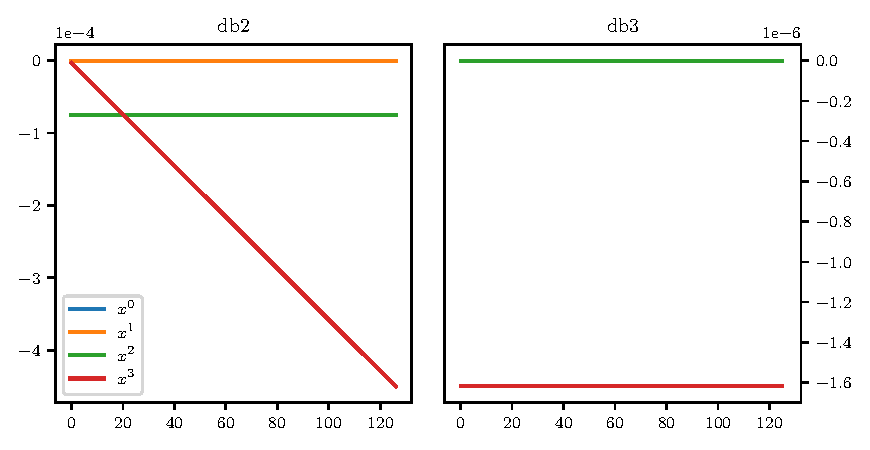
\includegraphics{papers/polynomials/images/polynomials_signals_db2_3.pdf}
    \caption{Analyse mit db2/3 Wavelet\label{polynomials:db2_3}}
\end{figure}

Wie sich herausstellt liefern diese Wavelets jeweils die zweite und dritte
Ableitung unserer Signale. Daubechies Wavelets mit $A$ verschwindenden Momenten
können uns also direkt die $A$-te Ableitung liefern. Dies im Gegensatz zum
Differenzieren welches mehrfach angewendet werden muss.

\section{Anwendung zur rauscharmen Ableitung}
\rhead{Rauscharme Ableitung}

Beim diskreten Ableiten (Differenzen) von Signalen stellt sich oftmals das
Problem, das Rauschen in dem Signal verstärkt wird. Anstelle der Ableitung des
interessanten Signals sehen wir also nur die zufällige Ableitung des Rauschens.
Dies wird nochmals verstärkt wenn ein Signal mehrfach abgeleitet werden soll.

\autoref{polynomials:noise:signals} zeigt unsere ursprünglichen polynomialen
Signale mit leichtem Rauschen versehen und die Ableitung davon. Wie erwartet
ist die Ableitung vom Rauschen dominiert und die Steigung des ursprünglichen
Polynoms ist kaum noch erkennbar.

\begin{figure}
    \centering
    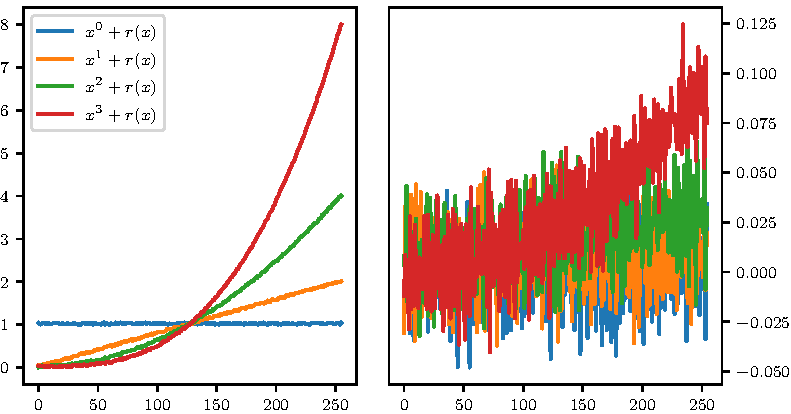
\includegraphics{papers/polynomials/images/polynomials_noise_signals.pdf}
    \caption{Verrauschte Signale und deren Ableitung\label{polynomials:noise:signals}}
\end{figure}

Was passiert nun wenn wir das verrauschte Signale mit einem Haar Wavelet
analysieren?  Wie in \autoref{polynomials:noise:db1} zu sehen bringt das so
noch keine wesentliche Verbesserung zum direkten Ableiten.

\begin{figure}
    \centering
    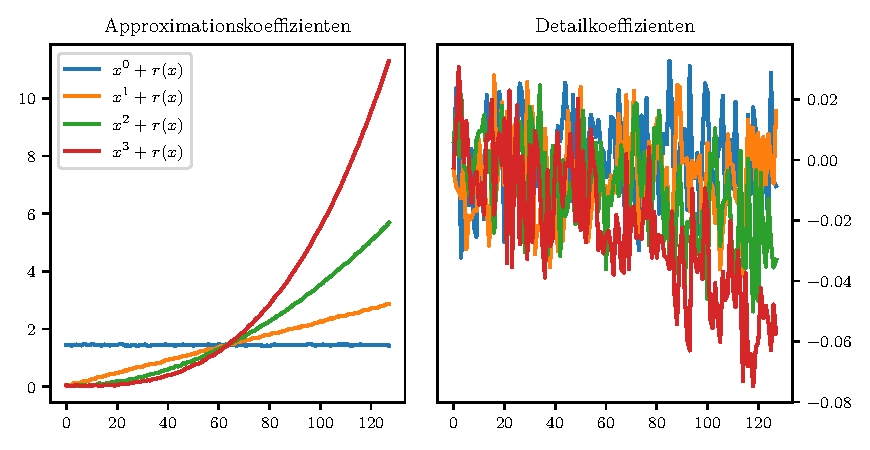
\includegraphics{papers/polynomials/images/polynomials_noise_db1.pdf}
    \caption{Analyse verrauschter Signale mit Haar Wavelet\label{polynomials:noise:db1}}
\end{figure}

Nun können wir aber mit dem Wavelet eine Multiskalenanalyse durchführen. Im
Fall vom Haar Wavelet ist dies vergleichbar wie wenn zuerst der Mittelwert
gebildet und dann abgeleitet wird. Aus \autoref{fast:akoefgleichung} von
\autoref{section:fast} wissen wir, dass die Approximationskoeffizienten $cA_{j,k}$ und die Detailkoeffizienten $dA_{j,k}$
folgendermassen gebildet werden:
\begin{align}
cA_{j+1,k}
&=
\frac{1}{\sqrt{2}} \sum_{l\in\mathbb Z} \bar{h}_l cA_{j,k+l}
\\
cD_{j+1,k}
&=
\frac{1}{\sqrt{2}} \sum_{l\in\mathbb Z} \bar{g}_l cA_{j,k+l}
\end{align}

Im Fall vom Haar-Wavelet enspricht das
\begin{align}
cA_{j+1,k}
&=
\frac{1}{\sqrt{2}} (cA_{j,k} + cA_{j,k+1})
\\
cD_{j+1,k}
&=
\frac{1}{\sqrt{2}} (cA_{j,k} - cA_{j,k+1})
\end{align}

Nehmen wir nun das Signal mit den Abtastwerten $\{a_{0,0}, a_{0,1}, a_{0,2}, a_{0,3}\}$ so ergibt
sich für die erste Ebene:
\begin{align}
cA_{1,0}
&=
\frac{1}{\sqrt{2}} (a_{0,0} + a_{0,1})
\\
cA_{1,1}
&=
\frac{1}{\sqrt{2}} (a_{0,2} + a_{0,3})
\end{align}
Die zweite Ebene wird dann aus den Approximationskoeffizienten der ersten Ebene berechnet
\begin{align}
cA_{2,0}
&=
\frac{1}{\sqrt{2}} (cA_{1,0} + cA_{1,1})
=
\frac{1}{2} (a_{0,0} + a_{0,1}) + \frac{1}{2} (a_{0,2} + a_{0,3})
\\
cD_{2,0}
&=
\frac{1}{\sqrt{2}} (cA_{1,0} - cA_{1,1})
=
\frac{1}{2} (a_{0,0} + a_{0,1}) - \frac{1}{2} (a_{0,2} + a_{0,3})
\end{align}

Die Detailkoeffizienten entsprechen somit der Differenz der Mittelwerte zweier
benachbarter Abtastwerte.

In \autoref{polynomials:noise:db1_multi} ist das Signal $x^2 + r(x)$, die
Detailkoeffizienten der verschiedenen Stufen der Multiskalenanalyse mit dem
Haar Wavelet und dann noch die Approximationskoeffizienten der letzten Stufe
abgebildet. Es ist zu sehen, dass die Detailkoeffizienten mit höherer Stufe
eher der Ableitung des originalen Polynoms entsprechen und weniger vom Rauschen
betroffen sind. Jedoch nimmt die zeitliche Auflösung ab.
Die Stufenbreite macht jeweils den zeitlichen Bereich, also die Anzahl Samples,
welcher für die Berechnung des jeweiligen Koeffizienten relevant ist sichtbar.

\begin{figure}
    \centering
    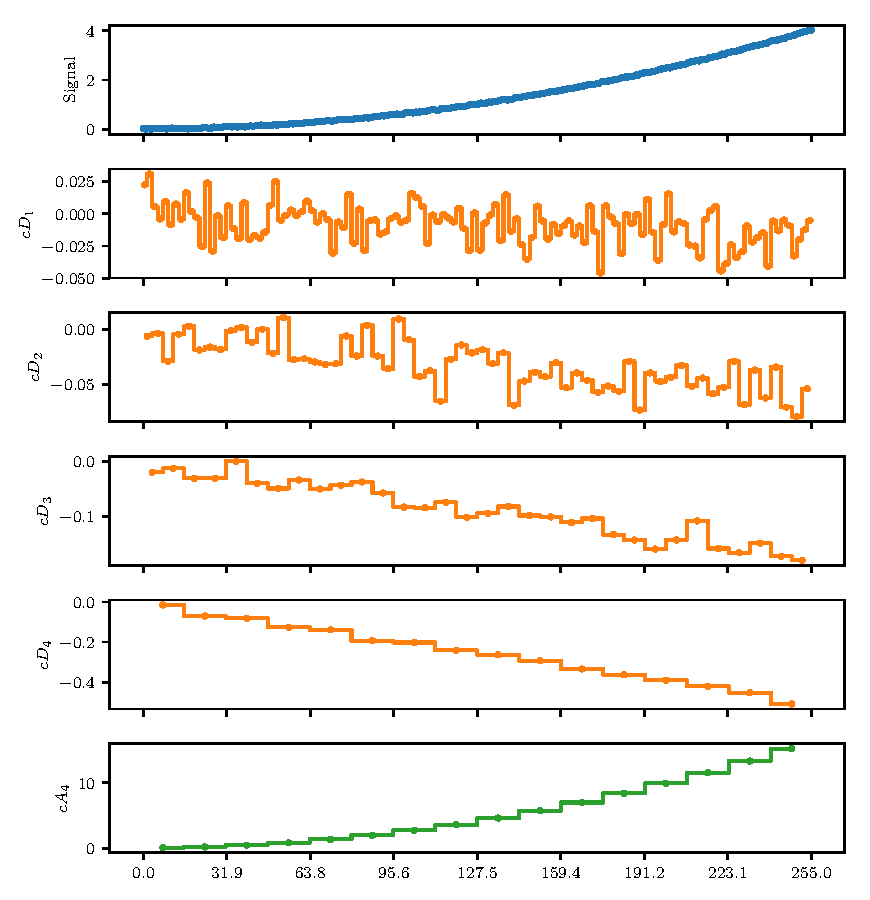
\includegraphics{papers/polynomials/images/polynomials_noise_db1_multi.pdf}
    \caption{Multiskalenanalyse von $x^2 + r(x)$ mit Haar Wavelet\label{polynomials:noise:db1_multi}}
\end{figure}

Im Vergleich dazu sind in \autoref{polynomials:noise:average} die direkte
Ableitung und die Ableitungen nach der Mittelwertbildung über 2, 4 und 8 Werte
zu sehen.

\begin{figure}
    \centering
    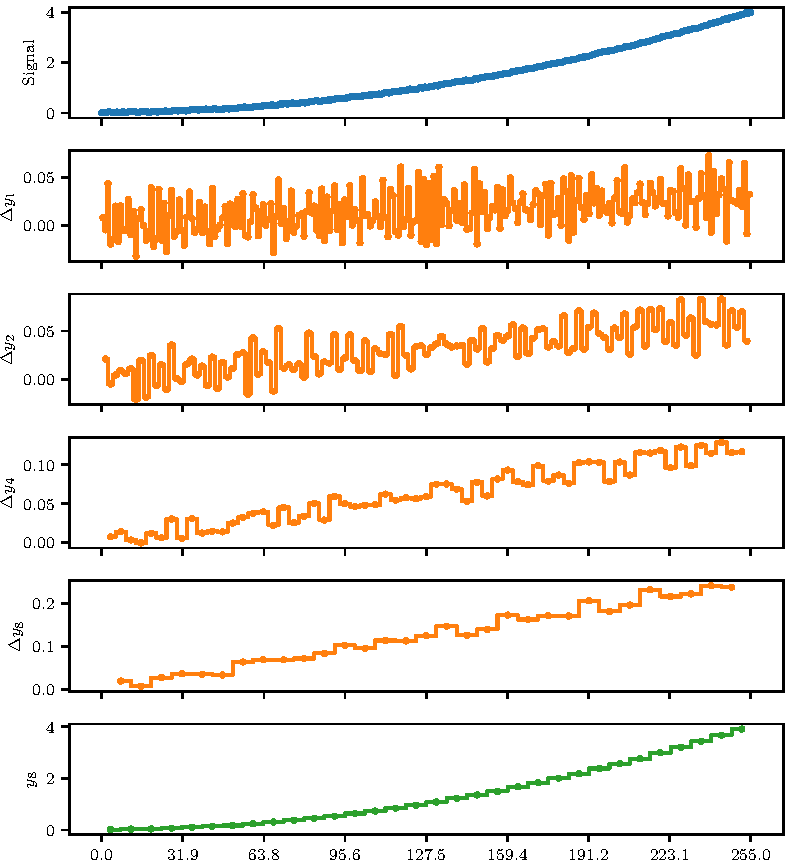
\includegraphics{papers/polynomials/images/polynomials_noise_moving_average.pdf}
    \caption{Ableitung nach Mittelwertbildung\label{polynomials:noise:average}}
\end{figure}

Nun haben wir aber mit dem Verfahren mit den Wavelets den Vorteil, dass wir bei
entsprechender Wahl des Wavelets mit $A$ verschwindenden Momenten direkt die
$A$-te Ableitung berechnen können.

In \autoref{polynomials:noise:db2_multi} ist das Signal $x^3 + r(x)$, die
Detailkoeffizienten der verschiedenen Stufen der Multiskalenanalyse mit dem db2
Wavelet und die Approximationskoeffizienten der letzten Stufe abgebildet.

\begin{figure}
    \centering
    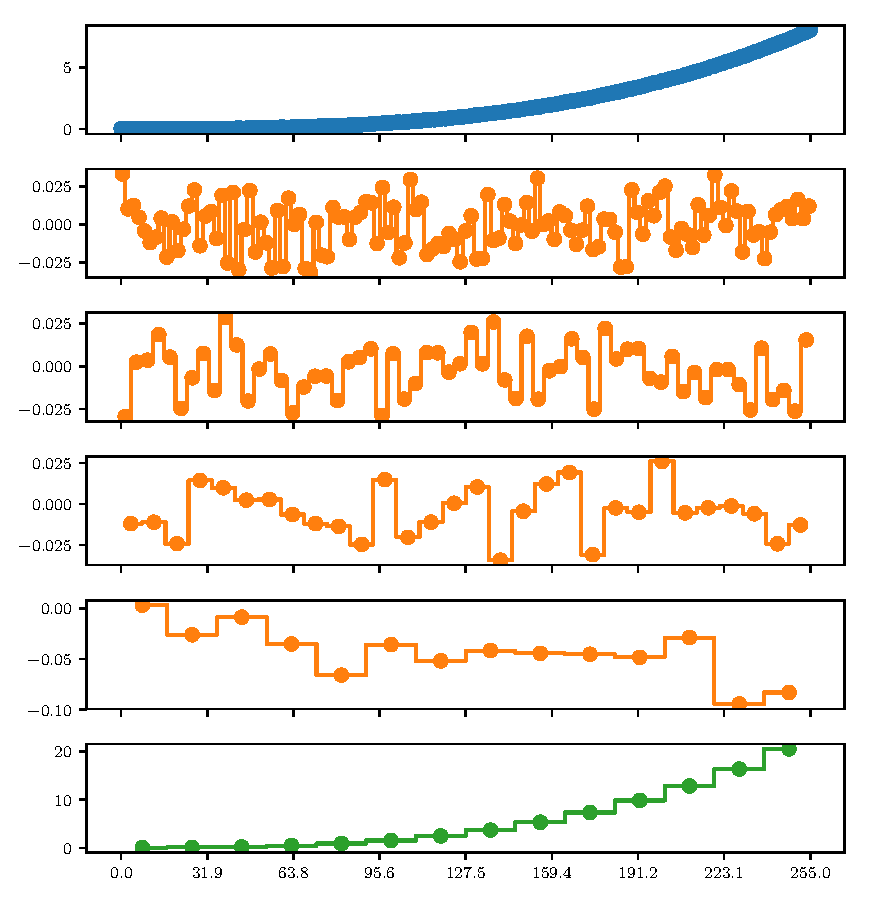
\includegraphics{papers/polynomials/images/polynomials_noise_db2_multi.pdf}
    \caption{Multiskalenanalyse von $x^3 + r(x)$ mit db2 Wavelet\label{polynomials:noise:db2_multi}}
\end{figure}

Im Vergleich dazu sind in \autoref{polynomials:noise:average} die direkt
berechnete zweite Ableitung und die zweite Ableitungen nach der
Mittelwertbildung über 2, 4 und 8 Werte zu sehen.

\begin{figure}
    \centering
    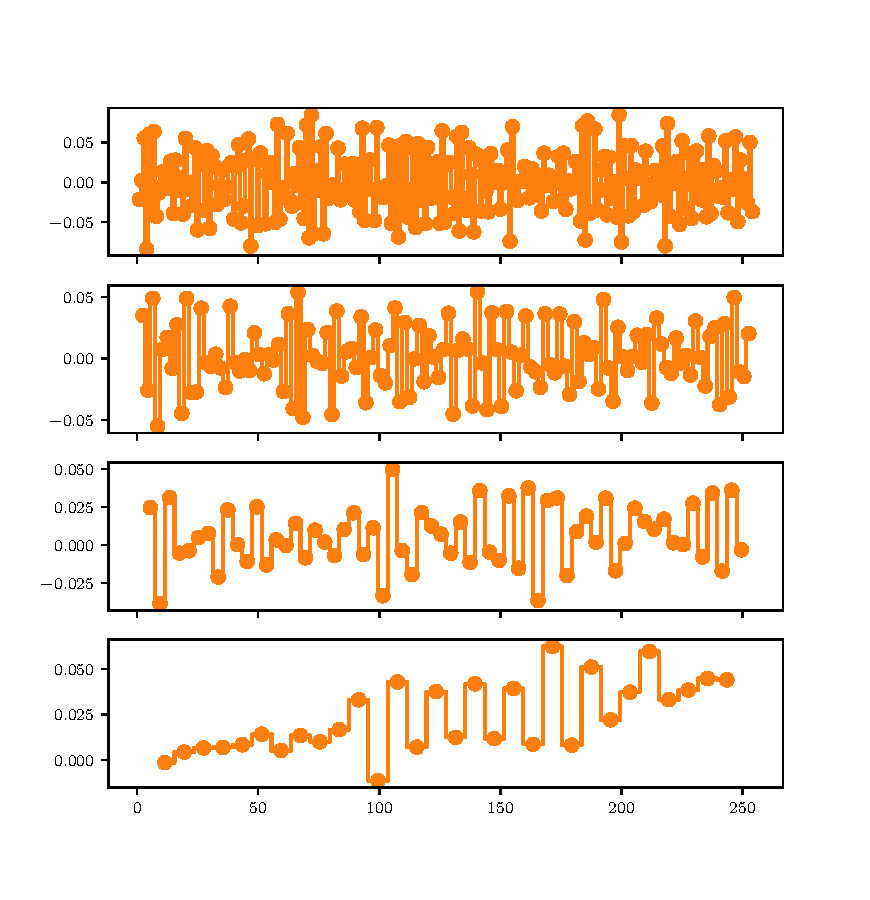
\includegraphics{papers/polynomials/images/polynomials_noise_moving_average_2nd.pdf}
    \caption{Zweite Ableitung nach Mittelwertbildung\label{polynomials:noise:average2nd}}
\end{figure}

Daubechies Wavelets bieten also eine komfortable Methode um verrauschte Signale
abzuleiten. Die Multiskalenanalyse kann dabei einen Kompromiss zwischen
Empfindlichkeit gegenüber Rauschen und zeitlicher Auflösung bieten.

Die Anwendung zur Ableitung kann auf der Binder Plattform im
\texttt{Ableitungen.ipynb} Notebook%
\footnote{\url{https://mybinder.org/v2/gh/rnestler/mathsem-FS2019/paper?filepath=Ableitungen.ipynb}}
nachvollzogen werden.

\section{Hochfrequente Anteile in Polynomen}
\rhead{Hochfrequente Anteile in Polynomen}

Im vorherigen Abschnitt waren wir vor allem an der Analyse des Polynoms und
dessen Ableitung interessiert. Die hochfrequenten Teile, also das Rauschen,
wollten wir dabei möglichst loswerden. Was nun aber wenn wir ein hochfrequentes
Signal aus einem sonst polynomialen Signal extrahieren wollen? Solche Signale
könnten zum Beispiel so wie in \autoref{polynomials:sin:signals} aussehen. Da
die Daubechies Wavelets polynomiale Signale schon komplett in den
Approximationskoeffizienten darstellen können, sollten wir das interessante
Signal direkt in den Detailkoeffizienten sehen können.

\begin{figure}
    \centering
    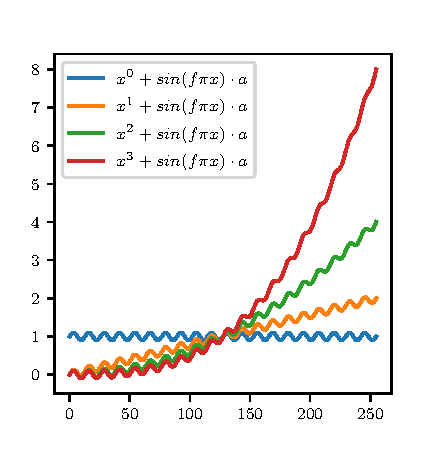
\includegraphics{papers/polynomials/images/polynomials_sin_signals.pdf}
    \caption{Polynomiale Signale mit Sinus\label{polynomials:sin:signals}}
\end{figure}

In \autoref{polynomials:sin:db2} ist die Analyse mit dem db2 Wavelet zu sehen.
Die Detailkoeffizienten werden von dem enthaltenen Sinussignal dominiert. Das
Sinussignal lässt sich also so bestens extrahieren.

\begin{figure}
    \centering
    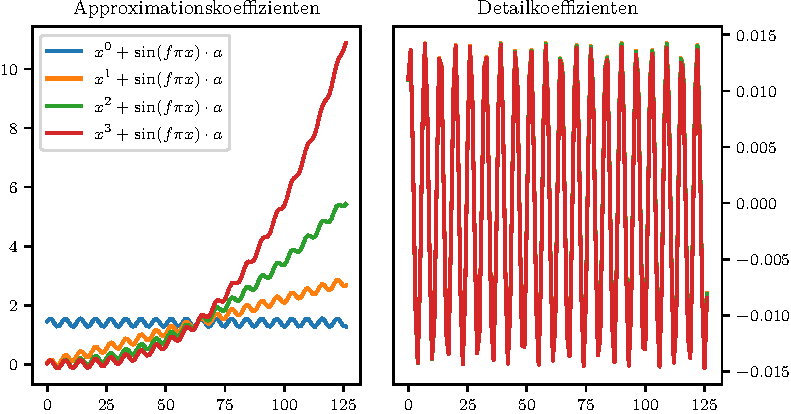
\includegraphics{papers/polynomials/images/polynomials_sin_db2.pdf}
    \caption{Analyse mit db2 Wavelet\label{polynomials:sin:db2}}
\end{figure}

Wenn man an sinusförmigen Signalen interessiert ist liegt es auch nahe die
diskrete Fourier Transformation zu verwenden. In \autoref{polynomials:sin:fft}
sind die Resultate der DFT zu sehen.

\begin{figure}
    \centering
    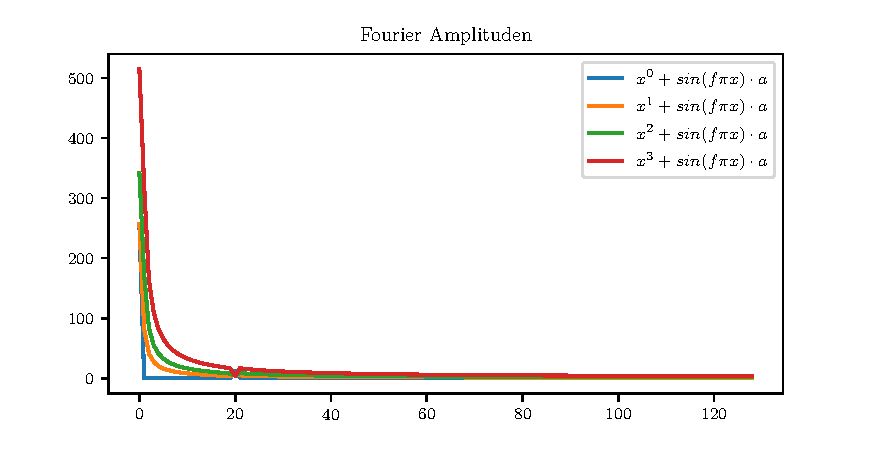
\includegraphics{papers/polynomials/images/polynomials_sin_fft.pdf}
    \caption{Analyse mit Fouriertransformation\label{polynomials:sin:fft}}
\end{figure}

Zu sehen ist, dass die Fourier Koeffizienten des Polynoms dominieren und dass
der Peak bei 20, welcher durch den Sinus entsteht, unter geht. Dies ist
verständlich, wenn man bedenkt wie die Fourierreihen von Polynomen aussehen.
Nehmen wir als Beispiel das Polynom $f(x) = x$. Im Bereich $[0, 1]$ entspricht
es einer Sägezahnfunktion. Die Fourier Reihe eines Sägezahns ist \[f(x) =
\frac{1}{2} - \frac{1}{\pi} \sum{\frac{1}{n} \sin(2 n \pi x)}\] Nun ist
ersichtlich, dass die Fouriertransformierte jede Frequenz $n$ mit $\frac{1}{n}$
skaliert enhalten wird.

Die Analyse mittels Fourier Transformation kann natürlich durch die Wahl einer
passenden Fensterfunktion (z.B. Hamming) zu besseren Resultaten führen. Dies
hat jedoch den Nachteil das zeitlich kurz auftretende Signale je nach
Fenstergrösse und Position unterschiedlich gedämpft werden.

Die Wavelettransformation liefert uns hingegen auch den Zeitpunkt bei dem das
Signal aufgetreten ist.  \autoref{polynomials:sin:padded} zeigt Die Resultate
einer Waveletanalyse mit einem zeitlich lokalisierten Sinussignal.

\begin{figure}
    \centering
    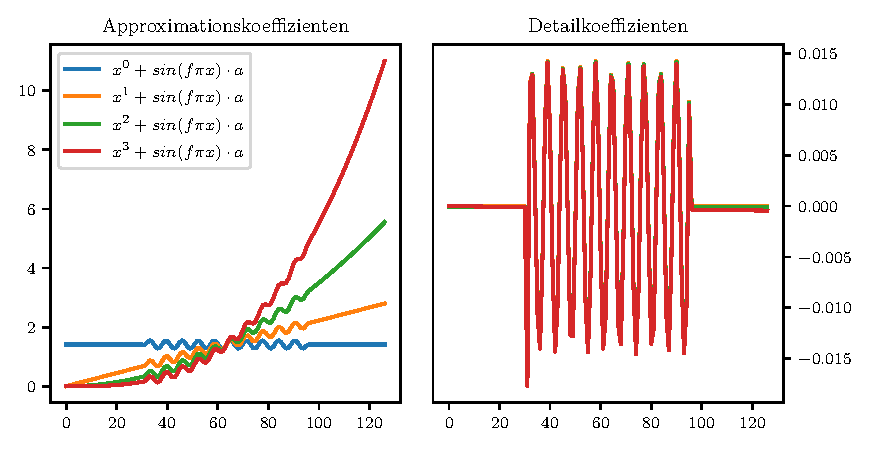
\includegraphics{papers/polynomials/images/polynomials_sin_padded_db2.pdf}
    \caption{Analyse mit db2 Wavelet eines zeitlich lokalisierten Sinuassignals\label{polynomials:sin:padded}}
\end{figure}

Die Analyse dieser Signale mit Daubechies Wavelets und DFT kann im
\texttt{Analyse von Sinus Signalen.ipynb} Notebook%
\footnote{\url{https://mybinder.org/v2/gh/rnestler/mathsem-FS2019/paper?filepath=Analyse\%20von\%20Sinus\%20Signalen.ipynb}}
nachvollzogen werden.

\section{Schlussfolgerung}
\rhead{Schlussfolgerung}

\printbibliography[heading=subbibliography]
\end{refsection}
